\documentclass[a4paper, 11pt]{article}
\usepackage{amsmath}
\usepackage{amssymb}
\usepackage[T1]{fontenc}
\usepackage[utf8x]{inputenc}
\usepackage{lmodern}
\usepackage{graphicx}
\graphicspath{ {./images/} }
\usepackage[english]{babel} 
\usepackage{natbib}
\usepackage{cite}
\usepackage[parfill]{parskip}
\usepackage{enumerate}
\usepackage{float}%for image positions
\usepackage{hyperref}
\hypersetup{
  colorlinks,
  citecolor=black,
  filecolor=black,
  linkcolor=black,
  urlcolor=black
}
\usepackage{amsthm}
\newtheorem{theorem}{Theorem}[section]
\newtheorem{lemma}[theorem]{Lemma}
\newtheorem{proposition}[theorem]{Proposition}
\newtheorem{axiom}[theorem]{Axiom}
\newtheorem{invariant}[theorem]{Invariant}
\newtheorem{breakpoint}[theorem]{Breakpoint}
\newtheorem{problem}{Problem}
\newtheorem{definition}{Definition} 
\usepackage{algorithm}
\usepackage{algpseudocode}
\usepackage{pifont}
\usepackage{multirow,array}
\usepackage{centernot}
\usepackage{comment} % enables the use of multi-line comments (\ifx \fi) 
\usepackage{lipsum} %This package just generates Lorem Ipsum filler text. 
\usepackage{fullpage} % changes the margin

\begin{document}
\section{Is Propagation Compositional?}
The two solution sets are identical which is shown by the program. Does this mean propagation is compositional?

Is there any other aspect in which they compute differently? In which aspect?

Propagation is not compositional, propagations communicate through the variables values and assignments. 

Yes they result in different search trees despite the fact that they are using the same search-heuristics (branching strategies):

First we have script $S1$ which models $A+B+C+B = X$ where $D_A = D_B = D_C = D_X = \{1,2,3,4,5\}$
\begin{figure}[H]
  \begin{center}
    \scalebox{0.90}{
      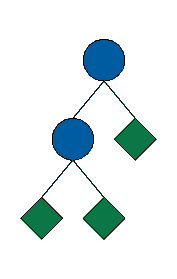
\includegraphics{first_fail_valmin_s1.pdf}
    }
    \caption{First-fail Minimum-value for Script S1}
    \label{fig:ffvms1}
  \end{center}
\end{figure}

Second we have script $S2$ which models $A+B = U; U+B+C = X$ where $D_A = D_B = D_C = D_X = D_U = \{1,2,3,4,5\}$
\begin{figure}[H]
  \begin{center}
    \scalebox{0.90}{
      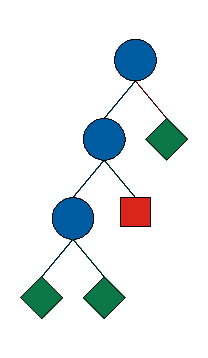
\includegraphics{first_fail_valmin_s2.pdf}
    }
    \caption{First-fail Minimum-value for Script S2}
    \label{fig:ffvms2}
  \end{center}
\end{figure}

What is happening?

In S1 we only post one constraint that will create propagators for that single constraint while in S2 there are two constraints posted. In the search tree of S2 the propagator for $A + B = U$ is executed first which results in interleaving of constraint propagation and variable assignment until the constraint is satisfied, in particular the assignments $A = 1, B = 2, U = 3$ is tried which leads to a (red) failed node since that means that there are no satisfying assignments for $C$ and $X$ that gives $U+B+C = X$. This is because $U+B=5$ and the maximum value of X is $5$ and the minimum value of $C$ is 1.

In S1 already before any assignment is made constraint propagation can infer that $B$ must be 1. This is the main difference. In S2 the constraint propagation were not able to resolve this initially since just looking at the constraint $U+B+C=X$ B could be other things than 1. But if the constraint propagation were able to consider both constraint simultaneously it would find out that $B$ could not be something else than 1, looking at each constraint in isolation $B$ does not have to be only 1.

\end{document}